\chapter{Modelo de Implementación}
\label{modelo_implementacion}

El modelo de implementación del SITEM esta compuesto básicamente por los siguientes artefactos que en su conjunto representan lo que comunmente se denomina el aplicativo:
\begin{itemize}
\item \textbf{Bloques:} Unidad Básica de funcionalidad. Se pueden pensar en ellos como “instancias” persistentes de clases abstractas. En especial se tienen tres clases:
\begin{itemize}
\item Administración: Con atributos y métodos para mostrar directorios de datos.
\item Menú: Con métodos especializados en la administración de enlaces dentro del SITEM.
\item Registro: Para la realización de casos CRUD.
\end{itemize}
\item \textbf{Clases}: Descriptores para varios tipos de objetos entre las cuales se tiene:
\begin{itemize}
\item DBMS: Interaccción con la bases de datos.
\item Página: Describe objetos que realizan la construcción en tiempo de ejecución de las páginas.
\item Encriptar: Descriptor para objetos que se encargan de codificar y decodificar los datos en el SITEM. El conjunto de operaciones debe ser manipulado en cada implementación del SITEM para garantizar un alto nivel de seguridad.
\item Autenticacion: Con descripción de atributos y operaciones que controlan las rutinas de AAA en el SITEM.
\item Config: Clasificador de objetos que manipulan las variables de configuración globales.
\item Html: Descriptor de controles de formularios en el SITEM.
\item Sesión: Operaciones y atributos para el control de sesiones en el SITEM luego del proceso de AAA.
\item Mensaje: Para objetos que administran mensajes de interacción con los actores.
\item Sql: Clase para describir objetos especializados en gestionar archivos con extensión SQL.
\item Navegacion: Con operaciones específicas para el control de desplazamiento entre conjuntos de registros.
\end{itemize}
\item \textbf{Función:} Métodos JavaScript para la validación y control de navegación en el lado del cliente.
\item \textbf{Estilo:} Para el control de la capa de Interfaz Gráfica.
\end{itemize}

\begin{figure}
 \centering
 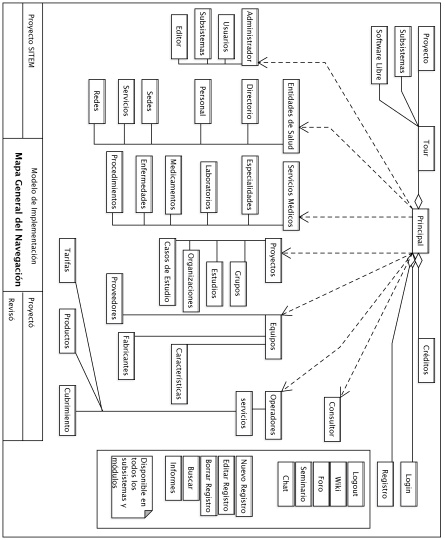
\includegraphics[width=156mm, height=182mm]{mapa_navegacion.png}
 \caption{Modelo General de Navegación}
 \label{mapa_navegacion}
\end{figure}

\section{Código Fuente del SITEM}

La siguiente porción de código fuente representa el formato general que se encuentra en el SITEM. Por patrón general se recomienda a todos los grupos que participan en el desarrollo que mantengan un esquema de codificación claro y documentación \textit{in situ} suficiente para aclarar secciones.

\subsection{Clase Página}

La clase Página tiene las operaciones:
\begin{itemize}
\item pagina: Constructor.
\item especificar pagina: Inicializar variables privadas.
\item procesar pagina: Controlar redireccionamientos.
\item ancho seccion: Implementa control de secciones colapsadas.
\item armar seccion: Para seleccionar los bloques que contiene cada página.
\end{itemize}

Algunos métodos instancian la clase DBMS y HTML. Estas por lo tanto deben ser visibles.
\begin{verbatim*}

class pagina
{

	//Metodo constructor
	function pagina(id_pagina,configuracion)
	{
		//Declaracion de variable parta controlar accesos indebidos
		GLOBALS["autorizado"]=TRUE;
		this->especificar_pagina(id_pagina);
		
		if(!isset(_POST['registro_compuesta']))
		{
			if(!isset(_REQUEST['action']))
			{
				
				this->mostrar_pagina(configuracion);
			}
			else
			{
				//echo 'Procesamiento de la pagina';
				this->procesar_pagina(configuracion);
			}
		}
		else
		{
			this->mostrar_pagina(configuracion);		
		}
	}
	//Fin del metodo constructor
	
	
	
	//Metodo especificar_pagina
	function especificar_pagina(id_pagina)
	{
	
		this->id_pagina=id_pagina;
	
	}
	//Fin del metodo especificar_pagina
.
.
.
} \end{verbatim*}